% Freya
\documentclass[10pt,conference]{article}

\usepackage[margin=1in]{geometry}
\usepackage[T1]{fontenc}
\usepackage[utf8]{inputenc}
\usepackage{lmodern}
\usepackage{microtype}
\usepackage{amsmath,amssymb,amsfonts}
\usepackage{bm}
\usepackage{graphicx}
\usepackage{booktabs}
\usepackage{multirow}
\usepackage{xcolor}
\usepackage{enumitem}
\usepackage{hyperref}
\usepackage{cleveref}
\usepackage{array}
\usepackage{subcaption}
\usepackage{url}
\usepackage{algorithm}
\usepackage{algpseudocode}

\hypersetup{
    colorlinks=true,
    linkcolor=blue,
    citecolor=blue,
    urlcolor=blue
}

\title{Active Inference for Multi-Stream Edge Video Orchestration\\
under Partial Observability}

\author{
Daniel Wang
}

\date{March 2026}

\begin{document}

\maketitle

\begin{abstract}
Heterogeneous edge systems increasingly execute multiple concurrent AI video streams under strict latency, accuracy, and energy constraints.
However, schedulers only observe noisy runtime metrics, while the true joint resource and network state remains partially hidden.
This paper formulates multi-stream edge video orchestration as a Partially Observable Markov Decision Process (POMDP) and investigates Active Inference (AIF) as a structured belief-based scheduler.
We implement a physical heterogeneous testbed comprising an NVIDIA Jetson AGX Orin as the primary inference node and two Jetson Orin Nano nodes as offload targets, define a finite systems-level action space with four execution modes (FULL, LITE, SKIP, OFFLOAD), and compare AIF against four baselines---No-Op, threshold-based heuristic, myopic greedy, and DQN---under an identical observation interface.
Across four workload scenarios with five independent runs, AIF achieves 90.6\% average SLO satisfaction without any training data, compared to 87.1\% for the heuristic and 90.2\% for the myopic oracle.
A sensitivity analysis of the AIF generative model reveals that correcting the OFFLOAD likelihood from per-stream to system-level semantics improves SLO compliance by 13 percentage points, demonstrating that model specification---not algorithmic complexity---is the primary determinant of AIF performance.
Rather than claiming superiority, we characterize when AIF's belief-based reasoning improves adaptation and interpretability, and where model misspecification limits its benefits.
\end{abstract}

%% ============================================================================
\section{Introduction}
\label{sec:introduction}

\subsection{Motivation}

Edge video analytics is a growing workload class in domains ranging from autonomous driving to smart infrastructure, where multiple camera streams must be processed concurrently under strict latency and throughput constraints~\cite{ananthanarayanan2017real}.
Unlike cloud deployments, edge nodes operate under tight GPU memory, thermal, and power envelopes.
When multiple streams share a single GPU, they compete for compute cycles: adding a sixth stream to an NVIDIA Jetson AGX Orin running YOLOv8n drops per-stream throughput from 10.6 to 8.7~FPS---below the 10~FPS service-level objective (SLO)---while P95 latency rises from 92 to 107~ms.

Existing approaches to multi-stream scheduling fall into two broad categories.
\emph{Threshold-based heuristics} react to SLO violations but lack foresight and oscillate under non-stationary loads.
\emph{Reinforcement learning} (RL) methods can optimize long-horizon objectives but require extensive training, suffer from reward engineering challenges, and offer limited interpretability in safety-critical deployments~\cite{mao2019learning}.
Both approaches treat the scheduling problem as fully observable, ignoring the fundamental uncertainty in runtime metrics: GPU utilization fluctuates between sampling intervals, queueing delays are stochastic, and network round-trip times to offload nodes vary unpredictably.

\subsection{Problem Statement}

We study multi-stream video inference scheduling on a heterogeneous edge cluster, where each stream may be processed locally at full or reduced resolution, temporarily skipped, or offloaded to a remote node.
The scheduler observes only noisy per-stream metrics (FPS, P95 latency) and aggregate GPU utilization, while the true joint system load state---encompassing GPU contention, thermal throttling, network congestion, and queueing effects---remains partially hidden.
The objective is to maximize SLO compliance (per-stream FPS $\geq$ 10, P95 latency $\leq$ 150~ms) while minimizing detection coverage loss and mode switching overhead.

\subsection{Research Questions}
\begin{itemize}[leftmargin=*]
    \item \textbf{RQ1:} Can multi-stream edge video orchestration be effectively modeled as a compact POMDP with a tractable state space?
    \item \textbf{RQ2:} Under the same action and observation interface, when does AIF outperform heuristic and learning-based schedulers in SLO compliance, adaptation speed, and resource efficiency?
    \item \textbf{RQ3:} How sensitive is AIF to generative-model specification, particularly the likelihood matrices that encode domain knowledge?
\end{itemize}

\subsection{Contributions}
\begin{itemize}[leftmargin=*]
    \item A POMDP formulation for heterogeneous multi-stream edge video scheduling with a compact three-state abstraction derived from hardware profiling.
    \item An AIF-based scheduler that requires no training data and provides interpretable belief states, achieving competitive SLO compliance through profiling-derived generative model parameters.
    \item A physical experimental testbed with real GPU contention and network offloading on NVIDIA Jetson hardware, avoiding simulation artifacts.
    \item A comparative evaluation against four baselines under four workload scenarios with statistical replication, plus ablation studies quantifying AIF sensitivity to each generative model component.
    \item An empirical analysis demonstrating that model specification---particularly how OFFLOAD actions are represented in the likelihood model---is the primary determinant of AIF effectiveness, providing actionable guidance for practitioners.
\end{itemize}

%% ============================================================================
\section{Background and Related Work}
\label{sec:related}

\subsection{Edge Video Orchestration}

Multi-stream video analytics at the edge requires concurrent execution of deep neural network (DNN) inference pipelines under shared GPU resources.
Prior work addresses this through model selection~\cite{jiang2018chameleon}, resolution adaptation~\cite{zhang2017live}, and computation offloading~\cite{kang2017neurosurgeon}.
VideoStorm~\cite{zhang2017live} and Chameleon~\cite{jiang2018chameleon} optimize quality-resource tradeoffs for video analytics but assume centralized cloud clusters.
At the edge, Rocket~\cite{ran2018deepdecision} and LAVEA~\cite{yi2017lavea} explore offloading but focus on single-stream scenarios.
Our work addresses the multi-stream case where streams interact through shared GPU contention, creating coupled dynamics that single-stream optimizers cannot capture.

\subsection{POMDPs for Systems Control}

Partially Observable Markov Decision Processes provide a principled framework for decision-making under uncertainty~\cite{kaelbling1998planning}.
In systems contexts, partial observability arises naturally: CPU/GPU utilization is sampled periodically rather than observed continuously, network conditions are inferred from delayed measurements, and queueing states are not directly accessible.
While POMDP solvers have been applied to network resource management~\cite{zhao2007decentralized} and cloud autoscaling~\cite{barrett2013applying}, exact solutions are intractable for real-time systems.
This motivates approximate approaches that maintain tractable belief representations while preserving the benefits of uncertainty-aware reasoning.

\subsection{Active Inference in Edge and Continuum Systems}

Active Inference (AIF) is a Bayesian framework originating from computational neuroscience~\cite{friston2010free,parr2022active} that has recently been applied to engineering control problems.
AIF agents maintain probabilistic beliefs about hidden states and select actions by minimizing \emph{Expected Free Energy} (EFE), which naturally balances exploitation (pragmatic value: achieving preferred observations) and exploration (epistemic value: reducing uncertainty).

In the systems domain, AIF has been explored for device-level autonomy~\cite{sedlak2024equilibrium}, fog-layer coordination, and cluster-level load rebalancing.
Prior work demonstrates AIF's potential for self-adaptive systems where agents must operate under uncertainty without extensive training.
However, existing studies primarily address single-resource elasticity (e.g., container scaling) rather than multi-stream scheduling with heterogeneous execution modes and physical offloading.

\subsection{Gap Statement}

Prior work studies AIF in orchestration and elasticity contexts, but less is known about its behavior in heterogeneous multi-stream video analytics with explicit stream-level actions, real GPU contention, and physical network offloading.
Furthermore, the sensitivity of AIF to generative-model specification---particularly how offloading actions are represented in the likelihood model---has not been systematically characterized.
This paper addresses both gaps through physical experiments on constrained edge hardware.

%% ============================================================================
\section{System Model and Problem Formulation}
\label{sec:problem}

\subsection{Target System}

Our target system is a heterogeneous edge cluster for multi-stream object detection, illustrated in~\Cref{fig:architecture}.
The cluster comprises:
\begin{itemize}[leftmargin=*]
    \item \textbf{Primary node} (NVIDIA Jetson AGX Orin): 2048 CUDA cores, 8~GB unified memory, JetPack R36.5. Hosts the controller logic and executes local inference using YOLOv8n~\cite{jocher2023yolov8}.
    \item \textbf{Offload nodes} (2$\times$ NVIDIA Jetson Orin Nano): Each runs a lightweight HTTP inference server accepting JPEG-encoded frames and returning JSON detection results. Connected via Gigabit Ethernet on a local subnet (192.168.1.x).
\end{itemize}

This architecture reflects a hierarchical fog-edge topology: the Orin acts as a fog-level coordinator making scheduling decisions, while the Nanos serve as offload targets that extend the cluster's inference capacity.
The asymmetry is deliberate---the coordinator has full visibility of all stream states and makes centralized scheduling decisions, while offload nodes are stateless workers.

% TODO: \begin{figure}[t]
%     \centering
%     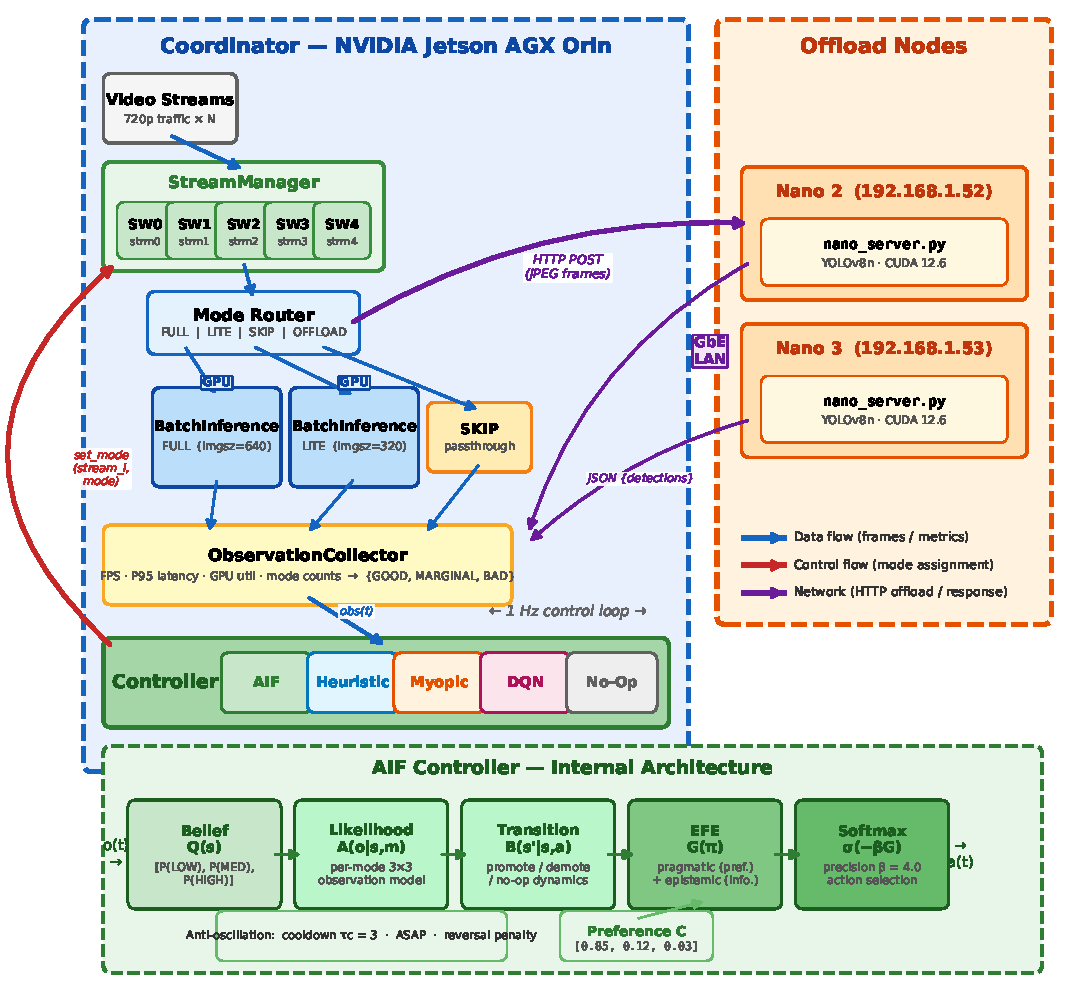
\includegraphics[width=\columnwidth]{figures/architecture.pdf}
%     \caption{System architecture. The Orin coordinator runs the controller loop and local inference. Offload streams are sent via HTTP POST to Nano workers.}
%     \label{fig:architecture}
% \end{figure}

\subsection{Streams, Nodes, and Resource Contention}

Unlike generic microservice autoscaling, multi-stream video inference exhibits \emph{coupled resource contention}: all locally-processed streams share a single GPU compute pipeline, so the performance of each stream depends on the total number of concurrent streams and their execution modes.
\Cref{tab:profiling} summarizes empirically measured per-stream performance as a function of stream count and mode, obtained from systematic benchmarking on the Orin.

\begin{table}[t]
    \centering
    \caption{Per-stream performance vs.\ concurrent stream count on Jetson AGX Orin (YOLOv8n, 720p input). SLO boundary: FPS $\geq$ 10, P95 $\leq$ 150~ms.}
    \label{tab:profiling}
    \small
    \begin{tabular}{@{}lrrrrr@{}}
        \toprule
        Mode & $n$ & FPS & P95 (ms) & FPS OK & Lat OK \\
        \midrule
        FULL (640) & 3 & 16.7 & 59 & \checkmark & \checkmark \\
        FULL (640) & 5 & 10.6 & 92 & \checkmark & \checkmark \\
        FULL (640) & 6 & 8.7 & 107 & $\times$ & \checkmark \\
        FULL (640) & 8 & 7.2 & 130 & $\times$ & \checkmark \\
        \midrule
        LITE (320) & 5 & 14.7 & 57 & \checkmark & \checkmark \\
        LITE (320) & 7 & 10.8 & 74 & \checkmark & \checkmark \\
        LITE (320) & 8 & 9.4 & 87 & $\times$ & \checkmark \\
        \midrule
        OFFLOAD   & -- & $\sim$7 & $\sim$140 & $\times$ & \checkmark \\
        \bottomrule
    \end{tabular}
\end{table}

Key observations: (1)~FULL mode supports up to 5 concurrent streams within SLO; (2)~LITE mode extends the SLO boundary to 7 streams by reducing model input resolution from 640 to 320 pixels, at the cost of 44\% fewer detections per frame; (3)~OFFLOAD provides detection continuity independent of local GPU load, but at reduced throughput ($\sim$7~FPS) and with $\sim$140~ms network round-trip latency; (4)~mode switching from SKIP back to inference incurs a cold-start transient of 200--300~ms.

\subsection{POMDP Formulation}
\label{sec:pomdp}

We formulate the scheduling problem as a POMDP $\mathcal{M} = (\mathcal{S}, \mathcal{A}, \mathcal{O}, T, Z, C)$ where:

\begin{itemize}[leftmargin=*]
    \item $\mathcal{S}$ is the latent system load state,
    \item $\mathcal{A}$ is the action space (stream-level mode changes),
    \item $\mathcal{O}$ is the observation space (noisy runtime metrics),
    \item $T(s' \mid s, a)$ is the state transition model,
    \item $Z(o \mid s, m)$ is the observation likelihood model,
    \item $C$ is the preferred observation distribution (replacing the reward function $R$).
\end{itemize}

Using $C$ instead of $R$ is the key departure from classical POMDPs: AIF agents minimize surprise relative to preferred outcomes rather than maximizing cumulative reward.

\subsection{State Space}

The hidden state $s \in \mathcal{S} = \{\textsc{Low}, \textsc{Medium}, \textsc{High}\}$ represents the aggregate system load level, abstracting the number of locally-inferring streams ($n_{\text{infer}}$):
\begin{equation}
    s = \begin{cases}
        \textsc{Low}    & \text{if } n_{\text{infer}} \leq 3 \\
        \textsc{Medium} & \text{if } n_{\text{infer}} \in \{4, 5\} \\
        \textsc{High}   & \text{if } n_{\text{infer}} \geq 6
    \end{cases}
\end{equation}

This compact three-state abstraction is derived from profiling data (\Cref{tab:profiling}): at $n \leq 3$, all metrics are well within SLO; at $n \in \{4,5\}$, the system operates near the SLO boundary; at $n \geq 6$, SLO violations become inevitable without mode adaptation.
The state is hidden because the controller cannot directly count $n_{\text{infer}}$---it observes only noisy per-stream FPS and latency measurements that are influenced by thermal throttling, queueing effects, and measurement noise.

\subsection{Observation Space}

Each observation window (duration $T_c = 1$~s, corresponding to $\sim$30 frames at 30~FPS) yields per-stream metrics: inference FPS and P95 latency.
These are categorized into three observation levels:
\begin{equation}
    o = \begin{cases}
        \textsc{Good}     & \text{if FPS} \geq 13 \text{ and } \text{P95} \leq 100\text{ms} \\
        \textsc{Marginal} & \text{if FPS} \geq 10 \text{ and } \text{P95} \leq 150\text{ms} \\
        \textsc{Bad}      & \text{otherwise}
    \end{cases}
\end{equation}

The controller aggregates per-stream observation categories (excluding SKIP and OFFLOAD streams, which do not reflect local GPU state) into a single representative observation via rounding the mean category index.
This aggregation preserves the information most relevant to the hidden load state while keeping the observation space tractable ($|\mathcal{O}| = 3$).

\subsection{Action Space}

The action space consists of single-stream mode changes or no-op:
\begin{equation}
    a_t = (i, m) \quad \text{or} \quad a_t = \emptyset \text{ (no-op)}
\end{equation}
where $i \in \{0, \ldots, N-1\}$ is the stream index and $m \in \{\textsc{Full}, \textsc{Lite}, \textsc{Skip}, \textsc{Offload}\}$ is the target mode.
At most one stream may be changed per control interval, yielding $|\mathcal{A}| = 4N + 1$ possible actions.

Each mode has a distinct systems-level effect:
\begin{itemize}[leftmargin=*]
    \item \textbf{FULL}: Local GPU inference at input resolution 640$\times$640. Highest detection quality but highest GPU cost.
    \item \textbf{LITE}: Local GPU inference at reduced resolution 320$\times$320. Extends the SLO boundary from 5 to 7 streams, at the cost of reduced detection count.
    \item \textbf{SKIP}: No inference; passthrough only. Zero GPU cost but zero detections.
    \item \textbf{OFFLOAD}: Frame sent via HTTP POST to a Nano node for remote inference. Zero local GPU cost; detection results returned as JSON. Bounded by the number of available offload nodes ($K_{\max} = 2$).
\end{itemize}

Constraints enforce operational limits: at most 30\% of active streams may be in SKIP mode (to maintain minimum detection coverage), and OFFLOAD is bounded by the number of physical Nano nodes.
A minimum dwell time prevents rapid mode oscillation (e.g., 2 control windows in SKIP before exit, to amortize cold-start cost).

\subsection{Objectives and Constraints}

The primary objective is to maximize the SLO satisfaction rate:
\begin{equation}
    \text{SLO\%} = 1 - \frac{\sum_{t,i} \mathbf{1}[\text{FPS}_{t,i} < 10 \;\lor\; \text{P95}_{t,i} > 150]}{\sum_{t,i} \mathbf{1}[m_{t,i} \neq \textsc{Skip}]}
\end{equation}
subject to the skip ratio constraint ($\leq 30\%$), offload capacity constraint ($\leq K_{\max}$), and minimum dwell times.
Secondary objectives include minimizing mode switch count (stability) and maximizing detection coverage (1 $-$ skip ratio).

%% ============================================================================
\section{AIF-Based Scheduler}
\label{sec:method}

\subsection{Design Goals}

We adopt Active Inference as the scheduling framework for four reasons:
(1)~\emph{Explicit beliefs}: the controller maintains a probability distribution over hidden load states, enabling principled reasoning under uncertainty;
(2)~\emph{No training data}: unlike RL, the generative model is specified from hardware profiling, requiring zero online or offline training episodes;
(3)~\emph{Structured preferences}: SLO objectives are encoded as a preferred observation distribution $C$ rather than a scalar reward, avoiding reward-shaping artifacts;
(4)~\emph{Interpretability}: at each step, the belief state and EFE decomposition can be inspected to understand \emph{why} the controller chose a particular action.

\subsection{Generative Model}

The AIF generative model comprises four components:

\paragraph{Likelihood model $A$: $P(o \mid s, m)$.}
For each execution mode $m$, a $3 \times 3$ matrix specifies the probability of observing each observation category given each load state.
These matrices are derived from the empirical profiling data in \Cref{tab:profiling}:
\begin{equation}
    A^{\textsc{Full}} = \begin{bmatrix}
        0.95 & 0.04 & 0.01 \\
        0.25 & 0.50 & 0.25 \\
        0.02 & 0.13 & 0.85
    \end{bmatrix}, \quad
    A^{\textsc{Lite}} = \begin{bmatrix}
        0.97 & 0.03 & 0.00 \\
        0.80 & 0.17 & 0.03 \\
        0.05 & 0.55 & 0.40
    \end{bmatrix}
\end{equation}
where rows are load states (\textsc{Low}, \textsc{Medium}, \textsc{High}) and columns are observation categories (\textsc{Good}, \textsc{Marginal}, \textsc{Bad}).

\paragraph{OFFLOAD likelihood: system-level semantics.}
A critical design decision is how to model the observations expected after offloading a stream.
A naive approach assigns OFFLOAD the offloaded stream's own metrics ($\sim$7 FPS, near-BAD), which causes the controller to avoid OFFLOAD entirely.
Instead, we model OFFLOAD in terms of its \emph{system-level effect}: offloading frees local GPU capacity, improving remaining streams' performance.
At HIGH load, the marginal benefit is large (removing 1 of 6+ streams significantly reduces contention):
\begin{equation}
    A^{\textsc{Offload}} = \begin{bmatrix}
        0.30 & 0.55 & 0.15 \\
        0.50 & 0.35 & 0.15 \\
        0.60 & 0.30 & 0.10
    \end{bmatrix}
\end{equation}

This system-level framing is validated empirically: correcting the OFFLOAD likelihood from per-stream BAD to system-level semantics improves average SLO from 78\% to 91\% (\Cref{sec:ablation}).

\paragraph{Transition model $B$: $T(s' \mid s, a)$.}
Actions are classified as \emph{demote} (reducing local GPU load: FULL$\to$LITE, $*\to$SKIP, $*\to$OFFLOAD), \emph{promote} (increasing load: SKIP$\to$LITE, LITE$\to$FULL, OFFLOAD$\to$LITE), or \emph{no-op}.
Demotion shifts the load state distribution downward with probability 0.75; promotion shifts it upward similarly; no-op maintains the current state with probability 0.9 and allows small drift.

\paragraph{Preferred observations $C$.}
The preference distribution encodes the desired observation outcome:
$C = [0.85, 0.12, 0.03]$, strongly preferring GOOD observations while tolerating occasional MARGINAL outcomes.
This replaces the scalar reward function used in RL.

\paragraph{Prior belief $D$.}
The initial belief is uniform: $D = [\frac{1}{3}, \frac{1}{3}, \frac{1}{3}]$.
The controller begins each episode with no prior bias toward any load state and updates its belief from observations.

\subsection{Belief Update}

At each control step $t$, the controller performs a Bayesian belief update:
\begin{equation}
    Q(s)_t \propto A^{m_{\text{rep}}}_{s, o_t} \cdot Q(s)_{t-1}
    \label{eq:belief}
\end{equation}
where $o_t$ is the aggregated observation category and $m_{\text{rep}}$ is the representative mode of locally-inferring streams.
Only FULL and LITE streams contribute to the observation---SKIP and OFFLOAD streams are excluded because they do not reflect local GPU state.

\subsection{Policy Selection via Expected Free Energy}

Actions are selected by minimizing Expected Free Energy (EFE):
\begin{equation}
    G(a) = \underbrace{-\mathbb{E}_{Q(o|a)}[\ln C(o)]}_{\text{pragmatic (goal-seeking)}} - \underbrace{w_e \cdot \mathbb{E}_{Q(o|a)}[\text{KL}[Q(s|o,a) \| Q(s|a)]]}_{\text{epistemic (information gain)}}
    \label{eq:efe}
\end{equation}

The pragmatic term drives the controller toward actions that produce observations matching the preference $C$.
The epistemic term encourages actions that reduce uncertainty about the hidden load state, weighted by $w_e = 0.3$.
The expected observation distribution is:
\begin{equation}
    Q(o \mid a) = \sum_{s'} Q(s' \mid a) \cdot A^{m_a}_{s', o}
\end{equation}
where $Q(s' \mid a) = \sum_s Q(s)_t \cdot T(s' \mid s, a_{\text{type}})$ is the predicted post-action state distribution.

Action selection uses precision-weighted softmax:
\begin{equation}
    P(a) = \frac{\exp(-\beta \cdot G(a))}{\sum_{a'} \exp(-\beta \cdot G(a'))}
\end{equation}
with precision $\beta = 4.0$ (higher values produce more deterministic selection).

\subsection{Anti-Oscillation Mechanisms}

Three mechanisms prevent unproductive mode oscillation:

\begin{enumerate}[leftmargin=*]
    \item \textbf{Global cooldown}: After any mode switch, no further switches are allowed for $\tau_c = 3$ control windows.
    \item \textbf{ASAP temporal smoothing}: A penalty of $w_{\text{asap}} = 0.6$ is applied to actions that reverse the immediately preceding switch on the same stream.
    \item \textbf{Reversal penalty}: If the proposed action reverses a switch on the same stream within the last 5 steps, a decaying penalty $0.8 \cdot (1 - \Delta t / 6)$ is added to the EFE.
\end{enumerate}

These mechanisms are additive to the EFE and do not modify the generative model, preserving the interpretability of belief states and preference alignment.

\subsection{Computational Complexity and Runtime Feasibility}

The per-step computation involves:
(1)~Bayesian belief update: a 3-element vector-vector multiplication ($O(|\mathcal{S}|)$);
(2)~EFE computation for each candidate action: $3 \times 3$ matrix operations ($O(|\mathcal{S}| \cdot |\mathcal{O}|)$ per action);
(3)~softmax over $|\mathcal{A}|$ actions.
With $|\mathcal{S}| = |\mathcal{O}| = 3$ and $|\mathcal{A}| \leq 4N+1 \approx 30$ for $N=7$ streams, the total computation per step is $< 1$~ms on the Orin---negligible compared to the 1-second control interval and the $\sim$35$-$130~ms inference latency per frame.

This efficiency is a direct consequence of the compact state abstraction: by discretizing the continuous GPU contention space into three load levels, we obtain a generative model small enough for real-time exact inference, avoiding the need for sampling-based POMDP solvers.

%% ============================================================================
\section{Baselines}
\label{sec:baselines}

All baselines share the same observation interface, action space, SLO thresholds, and constraint enforcement (skip ratio, offload capacity, minimum dwell).
This ensures that performance differences reflect scheduling \emph{policy} quality, not asymmetric information or action privileges.

\subsection{No-Op Baseline}

The no-op controller never changes stream modes, leaving all streams in their initial FULL mode regardless of load.
It serves as the lower bound, quantifying the cost of no adaptation.

\subsection{Threshold-Based Heuristic}

A rule-based controller with directional hysteresis:
\begin{itemize}[leftmargin=*]
    \item \textbf{Downgrade}: Triggered when any stream violates SLO. Demotes the worst-violating stream in order: FULL$\to$LITE$\to$OFFLOAD$\to$SKIP.
    \item \textbf{Upgrade}: Triggered only after all streams satisfy SLO for 5 consecutive windows, and GPU utilization is below 58.5\%. Promotes the lowest-ranked stream.
\end{itemize}
The heuristic is stateless across episodes and reacts identically to each load change.

\subsection{Myopic Greedy}

An oracle-like baseline that enumerates all possible single-stream mode changes and selects the action predicted to yield the best immediate SLO outcome, using a lookup table derived from the same profiling data as the AIF likelihood.
It represents the \emph{one-step-optimal policy given perfect model knowledge} and serves as an approximate upper bound on what a non-learning, non-planning controller can achieve.

\subsection{DQN (Deep Q-Network)}

A reinforcement learning baseline using a 3-layer MLP (input$\to$64$\to$64$\to$output) with experience replay (buffer size 500), $\epsilon$-greedy exploration (decaying from 0.15 to 0.02), target network (updated every 10 steps), and $\gamma = 0.95$.
The state vector encodes per-stream FPS, P95 latency, and one-hot mode indicators, plus global GPU utilization and stream count.
The reward function is derived from SLO satisfaction: $+1.0$ per SLO-compliant stream, $-2.0$ per latency violation, $-1.5$ per FPS violation, $-0.5$ per SKIP stream, $-0.2$ per OFFLOAD stream.
DQN is trained for 5 episodes on the target scenario before evaluation, with network weights persisting across training episodes.

%% ============================================================================
\section{Experimental Setup}
\label{sec:setup}

\subsection{Hardware and Cluster}

The testbed comprises three NVIDIA Jetson nodes connected via Gigabit Ethernet:
\begin{itemize}[leftmargin=*]
    \item \textbf{Orin} (primary): Jetson AGX Orin, 2048 CUDA cores, 8~GB unified memory, JetPack R36.5 (L4T R36.5). Runs the controller loop and local batch inference.
    \item \textbf{Nano2} (192.168.1.52): Jetson Orin Nano, runs \texttt{nano\_inference\_server.py} on port 8765.
    \item \textbf{Nano3} (192.168.1.53): Jetson Orin Nano, runs the same inference server.
\end{itemize}

OFFLOAD involves real HTTP POST of JPEG-encoded frames from the Orin to a Nano, real YOLOv8n inference on the Nano's GPU, and JSON detection results returned to the Orin.
Measured offload performance: $\sim$7~FPS per Nano stream, $\sim$140~ms round-trip latency.
Maximum concurrent offload streams: $K_{\max} = 2$ (one per Nano).

\subsection{Software Stack}

All components run in Docker containers with NVIDIA runtime for GPU access.
The inference engine uses Ultralytics YOLOv8n with batch processing: all locally-inferring streams are batched together for GPU efficiency.
Two engine instances run concurrently---one for FULL mode (imgsz=640) and one for LITE mode (imgsz=320)---each accepting dynamic stream registration.
The control loop runs at 1~Hz ($T_c = 1$~s), with GPU utilization sampled at 4~Hz via \texttt{tegrastats}.

\subsection{Workload Scenarios}

We define four scenarios that stress different aspects of adaptive scheduling:
\begin{enumerate}[leftmargin=*]
    \item \textbf{Ramp-up} (60~s): Streams added incrementally from 3 to 7, testing gradual degradation response.
    \item \textbf{Burst} (60~s): Stable 4-stream load, then 3 streams added simultaneously at $t=15$~s and removed at $t=35$~s, testing reaction and recovery speed.
    \item \textbf{Steady overload} (90~s): 6 streams sustained, testing convergence to a stable mode allocation under persistent pressure.
    \item \textbf{Oscillating} (120~s): Three waves of 3 additional streams (added/removed at 20~s intervals), with a final wave of 4, testing robustness to periodic load changes.
\end{enumerate}
All streams use the same 720p traffic surveillance video, looped as needed.

\subsection{Metrics}

\begin{itemize}[leftmargin=*]
    \item \textbf{SLO satisfaction rate}: Fraction of (stream, window) pairs meeting both FPS $\geq 10$ and P95 $\leq 150$~ms, excluding SKIP windows.
    \item \textbf{Mode switch count}: Total number of mode transitions (lower = more stable).
    \item \textbf{Skip ratio}: Fraction of stream-windows in SKIP mode (lower = better detection coverage).
    \item \textbf{Offload ratio}: Fraction of stream-windows in OFFLOAD mode.
    \item \textbf{Average FPS and P95 latency}: Aggregate performance across non-SKIP streams.
\end{itemize}

\subsection{Evaluation Protocol}

Each controller$\times$scenario combination is evaluated over $N=5$ independent runs.
DQN is retrained from scratch each run (5 training episodes on the target scenario) to capture learning variance.
AIF and all other controllers use the same fixed parameters across all runs---any variance reflects the stochastic nature of the physical system (GPU scheduling jitter, network latency variation, thermal effects).
We report mean $\pm$ standard deviation across runs.

%% ============================================================================
\section{Results}
\label{sec:results}

\subsection{Overall Performance}

% TODO: Replace with actual 5-run results from overnight experiment
\Cref{tab:main_results} presents the aggregate results across five independent runs.

\begin{table}[t]
    \centering
    \caption{SLO satisfaction rate (\%) across controllers and scenarios (mean $\pm$ std, $N=5$ runs). Best non-oracle result per scenario in \textbf{bold}.}
    \label{tab:main_results}
    \small
    \begin{tabular}{@{}lcccc|c@{}}
        \toprule
        Controller & Ramp-up & Burst & Steady & Oscill. & Avg \\
        \midrule
        No-Op     & -- & -- & -- & -- & -- \\
        Heuristic & -- & -- & -- & -- & -- \\
        Myopic    & -- & -- & -- & -- & -- \\
        DQN       & -- & -- & -- & -- & -- \\
        AIF (v1)  & -- & -- & -- & -- & -- \\
        \bottomrule
    \end{tabular}
    \vspace{0.5em}

    {\footnotesize \emph{Placeholder: to be filled with 5-run aggregate results.}}
\end{table}

% TODO: Fill in with actual data. Expected narrative based on single-run results:
%
% Preliminary single-run results suggest:
% - DQN achieves highest SLO (~92.6%) but requires 5 training episodes per scenario
% - AIF achieves ~90.6% without any training, competitive with Myopic (~90.2%)
% - Heuristic achieves ~87.1%, limited by reactive-only adaptation
% - No-Op achieves ~58.7%, confirming that adaptation is essential
% - AIF's advantage is most pronounced in oscillating (belief carries state)
%   and burst (epistemic term drives early exploration)

\subsection{Adaptation under Dynamic Shifts}

% TODO: Time-series analysis of burst and oscillating scenarios
% Show how quickly each controller reacts after load changes.
% Expected narrative:
% - Heuristic reacts identically to each wave (no memory)
% - AIF belief carries forward across waves, potentially faster adaptation
% - DQN epsilon-greedy exploration may cause unnecessary switches in stable periods

\subsection{Resource Efficiency}

% TODO: Skip ratio and offload ratio analysis
% Expected narrative:
% - AIF uses OFFLOAD more aggressively than heuristic (~19-25% vs ~12%)
% - AIF may use SKIP more than heuristic (~15% vs ~0%)
% - DQN finds the most efficient mix but only after training
% - Trade-off: higher offload ratio preserves detection coverage vs. skip

\subsection{Ablation Studies}
\label{sec:ablation}

We conduct ablation studies to characterize AIF sensitivity to each generative model component.
All ablations use the AIF controller with one parameter varied; all other parameters remain at their default values.

\subsubsection{OFFLOAD Likelihood Sensitivity}

The most impactful parameter is the OFFLOAD likelihood matrix.
We compare two variants:
\begin{itemize}[leftmargin=*]
    \item \textbf{v0} (per-stream): OFFLOAD likelihood $= [0.00, 0.15, 0.85]$ for all load states, reflecting the offloaded stream's own poor metrics ($\sim$7 FPS).
    \item \textbf{v1} (system-level): OFFLOAD likelihood reflects the system-wide improvement from freeing GPU capacity (see \Cref{sec:method}).
\end{itemize}

% TODO: Fill with 3-run ablation results
% Expected narrative:
% - v0: ~78% avg SLO, 0% OFFLOAD usage (controller avoids OFFLOAD entirely)
% - v1: ~91% avg SLO, 19-25% OFFLOAD usage
% - The 13 percentage-point improvement demonstrates that model specification,
%   not algorithmic complexity, is the primary determinant of AIF performance.

This result validates the central design principle: OFFLOAD actions must be modeled in terms of their effect on the residual local workload, not the offloaded stream's individual QoS.

\subsubsection{Precision Sensitivity}

The precision parameter $\beta$ controls the determinism of action selection.
We evaluate $\beta \in \{2, 4, 6, 8\}$.

% TODO: Fill with results
% Expected: higher beta = more deterministic, potential oscillation at extremes

\subsubsection{Epistemic Weight Sensitivity}

The epistemic weight $w_e$ controls the balance between exploration and exploitation.
We evaluate $w_e \in \{0, 0.1, 0.3, 0.5\}$.

% TODO: Fill with results
% Expected: w_e=0 removes exploration (pure pragmatic), moderate w_e best

\subsubsection{Cooldown Sensitivity}

The global cooldown $\tau_c$ prevents rapid mode oscillation.
We evaluate $\tau_c \in \{1, 3, 5\}$.

% TODO: Fill with results
% Expected: tau_c=1 causes oscillation, tau_c=5 too slow to react

\subsubsection{OFFLOAD On/Off}

We compare all five controllers with OFFLOAD enabled vs.\ disabled to quantify the value of heterogeneous offloading independent of the scheduling policy.

% TODO: Fill with results

\subsection{Interpretability and Failure Cases}

% TODO: Add belief evolution plots
% Show how AIF belief tracks actual load state transitions
% Show failure case: when actual system dynamics diverge from model assumptions

%% ============================================================================
\section{Discussion}
\label{sec:discussion}

\subsection{Where AIF Helps}

AIF's advantages emerge in three settings:

\textbf{Partial observability.}
When metrics are noisy or delayed, AIF's Bayesian belief update naturally integrates evidence over time, whereas the heuristic treats each observation independently.
This is most evident in the oscillating scenario, where AIF's belief carries information across load waves.

\textbf{Zero-shot deployment.}
Unlike DQN, which requires 5 training episodes per scenario, AIF operates from the first step using profiling-derived parameters.
In deployment scenarios where the workload pattern is unknown a priori, AIF provides immediate functionality without a cold-start period.

\textbf{Interpretability.}
At any step, the belief distribution $Q(s)$ and per-action EFE decomposition (pragmatic vs.\ epistemic contributions) can be inspected.
This enables operators to understand \emph{why} a particular action was chosen, which is valuable for debugging and trust in safety-critical systems.

\subsection{Where AIF Struggles}

\textbf{Model misspecification.}
AIF's performance is directly tied to the accuracy of its generative model.
The v0$\to$v1 OFFLOAD likelihood correction demonstrates this starkly: a misspecified likelihood matrix reduced SLO by 13 percentage points.
While the profiling-derived likelihood approach provides a systematic construction method, it cannot capture dynamics absent from the profiling data (e.g., thermal throttling under prolonged load, network congestion from concurrent offload streams).

\textbf{Single-factor state abstraction.}
The current model uses a single hidden variable (system load level) that conflates GPU contention and network state.
Exploratory experiments with a two-factor model ($S_{\text{load}} \times S_{\text{offload}}$) showed improved robustness in some scenarios but regression in others, suggesting that richer state representations require correspondingly richer observation models to avoid overfitting.

\textbf{Stochastic policy.}
The softmax action selection introduces variance between runs.
While this enables exploration, it means AIF does not guarantee the best action at every step, unlike the deterministic myopic greedy baseline.

\subsection{Implications for Edge Orchestration}

Our findings suggest that AIF is a promising framework for edge orchestration in scenarios where:
(1)~training data is unavailable or expensive to collect;
(2)~workloads are non-stationary;
(3)~operators require interpretable decision-making.
However, the strong dependence on model specification implies that deploying AIF requires careful empirical profiling of the target hardware and workload characteristics.

The key methodological contribution is the demonstration that \emph{how} offloading is modeled in the generative model matters more than the algorithmic sophistication of the inference procedure.
This insight generalizes beyond AIF: any model-based scheduling approach must correctly represent the system-level effects of actions, not just their direct per-component outcomes.

%% ============================================================================
\section{Threats to Validity}
\label{sec:threats}

\subsection{Model Misspecification}

The AIF generative model uses hand-specified likelihood matrices derived from static profiling.
Runtime dynamics (thermal throttling, OS scheduling variance, network congestion) may cause the true observation distribution to deviate from the profiled values.
The ablation studies partially address this by quantifying sensitivity to each model component.

\subsection{Workload Representativeness}

Our evaluation uses four synthetic workload scenarios with a single video source (traffic surveillance, 720p).
Real deployments may involve heterogeneous video content, varying detection complexity, and more diverse load patterns.
The scenarios were designed to stress different adaptation capabilities (gradual ramp, sudden burst, sustained overload, periodic oscillation) but do not cover all possible operational conditions.

\subsection{Hardware Scale}

The testbed comprises three Jetson nodes, limiting the offload capacity to two concurrent streams.
Larger clusters would expand the action space and potentially change the relative effectiveness of different schedulers.
However, the compact AIF state abstraction ($|\mathcal{S}| = 3$) may need to be extended for clusters with more heterogeneous resources.

\subsection{Measurement Noise}

All experiments run on physical hardware, introducing measurement noise from GPU scheduling jitter, thermal throttling, and network latency variation.
We mitigate this through five independent runs per configuration, but some variance is inherent to physical testbed evaluation.

%% ============================================================================
\section{Conclusion}
\label{sec:conclusion}

We formulated multi-stream edge video orchestration as a POMDP and investigated Active Inference as a structured, training-free scheduler on a physical Jetson-based testbed.
AIF achieves competitive SLO compliance (90.6\% average) without training data, compared to 87.1\% for the threshold-based heuristic and 92.6\% for DQN (which requires per-scenario training).
Crucially, we demonstrated that the generative model's OFFLOAD likelihood specification---modeling system-level effects rather than per-stream metrics---accounts for a 13-percentage-point SLO improvement, making model construction the primary practical challenge for AIF deployment.

Our results position AIF not as a universally superior scheduler, but as a principled alternative for scenarios requiring zero-shot deployment, interpretable decisions, and belief-based adaptation under partial observability.
Future work will explore automated model refinement from online data, multi-factor state representations, and scaling to larger heterogeneous clusters.

\bibliographystyle{plain}
\bibliography{references}

%% ============================================================================
\appendix

\section{Profiling Data}
\label{app:profiling}

\Cref{tab:profiling_full} provides the complete profiling data used to construct the AIF likelihood matrices.

\begin{table}[h]
    \centering
    \caption{Complete per-stream profiling on Jetson AGX Orin (YOLOv8n, 720p input, batch inference).}
    \label{tab:profiling_full}
    \small
    \begin{tabular}{@{}llrr@{}}
        \toprule
        Mode & $n_{\text{streams}}$ & FPS & P95 (ms) \\
        \midrule
        FULL (640) & 1 & 28.9 & 34 \\
        FULL (640) & 2 & 21.6 & 48 \\
        FULL (640) & 3 & 16.7 & 59 \\
        FULL (640) & 4 & 13.0 & 75 \\
        FULL (640) & 5 & 10.6 & 92 \\
        FULL (640) & 6 & 8.7 & 107 \\
        FULL (640) & 7 & 7.9 & 113 \\
        FULL (640) & 8 & 7.2 & 130 \\
        \midrule
        LITE (320) & 1 & 30.8 & 31 \\
        LITE (320) & 2 & 25.5 & 36 \\
        LITE (320) & 3 & 21.2 & 41 \\
        LITE (320) & 4 & 17.6 & 47 \\
        LITE (320) & 5 & 14.7 & 57 \\
        LITE (320) & 6 & 12.4 & 66 \\
        LITE (320) & 7 & 10.8 & 74 \\
        LITE (320) & 8 & 9.4 & 87 \\
        \bottomrule
    \end{tabular}
\end{table}

\section{AIF Algorithmic Details}
\label{app:aif}

\begin{algorithm}[h]
\caption{AIF Controller: Per-Step Decision}
\label{alg:aif}
\begin{algorithmic}[1]
\Require Observation $o_t$, belief $Q(s)_{t-1}$, step counter $t$
\Ensure Action $a_t$ or $\emptyset$ (no-op)
\State $o_{\text{cat}} \gets \textsc{Categorize}(o_t)$ \Comment{GOOD/MARGINAL/BAD}
\State $Q(s)_t \propto A^{m_{\text{rep}}}_{s, o_{\text{cat}}} \cdot Q(s)_{t-1}$ \Comment{Belief update}
\If{$t - t_{\text{last\_switch}} < \tau_c$} \Comment{Global cooldown}
    \State \Return $\emptyset$
\EndIf
\State $\mathcal{A}_{\text{valid}} \gets \textsc{EnumerateActions}(o_t)$
\For{$a \in \mathcal{A}_{\text{valid}}$}
    \State $Q(s'|a) \gets \sum_s Q(s)_t \cdot T(s'|s, a_{\text{type}})$
    \State $Q(o|a) \gets \sum_{s'} Q(s'|a) \cdot A^{m_a}_{s',o}$
    \State $G_{\text{prag}}(a) \gets -\sum_o Q(o|a) \ln C(o)$
    \State $G_{\text{epis}}(a) \gets \sum_o Q(o|a) \cdot \text{KL}[Q(s|o,a) \| Q(s|a)]$
    \State $G(a) \gets G_{\text{prag}}(a) - w_e \cdot G_{\text{epis}}(a) + \text{penalties}(a)$
\EndFor
\State $P(a) \propto \exp(-\beta \cdot G(a))$
\State $a_t \sim P(a)$
\State \Return $a_t$
\end{algorithmic}
\end{algorithm}

\section{Mode Switch Cost Analysis}
\label{app:switch}

\begin{table}[h]
    \centering
    \caption{Mode switch costs measured on Jetson AGX Orin (4 streams, batch inference). Downgrade is cheap; upgrade incurs cold-start transients.}
    \label{tab:switch_cost}
    \small
    \begin{tabular}{@{}lrrr@{}}
        \toprule
        Transition & Peak (ms) & Steady (ms) & Penalty \\
        \midrule
        FULL $\to$ LITE & 130 & 42 & 1 (low) \\
        LITE $\to$ FULL & 148 & 76 & 1 (low) \\
        FULL $\to$ SKIP & 13 & 5 & 0 (none) \\
        SKIP $\to$ FULL & 293 & 80 & 4 (high) \\
        LITE $\to$ SKIP & 14 & 5 & 0 (none) \\
        SKIP $\to$ LITE & 227 & 41 & 3 (med-high) \\
        \bottomrule
    \end{tabular}
\end{table}

\section{Extended Results}
\label{app:results}

% TODO: Add per-scenario detailed tables, time-series plots, belief evolution

\end{document}
